\documentclass[tikz,border=8pt]{standalone}
% Shared look for every TikZ diagram. Load with \input{../../tools/tikz-style.tex}
\usepackage[T1]{fontenc}
\usepackage{lmodern}
\renewcommand{\sfdefault}{lmr}  % diagrams use the same serif as the text
\usetikzlibrary{arrows.meta, positioning, shapes.geometric, calc, fit, backgrounds}
\definecolor{cblue}{HTML}{4C78A8}
\definecolor{corange}{HTML}{F58518}
\definecolor{cgreen}{HTML}{54A24B}
\definecolor{cred}{HTML}{E45756}
\definecolor{cpurple}{HTML}{B279A2}
\definecolor{cgrey}{HTML}{6B6B6B}
\tikzset{
  every picture/.style={font=\sffamily, line width=1.2pt},
  box/.style={draw=#1, fill=#1!12, rounded corners=4pt, align=center, inner sep=7pt, minimum height=1.1cm},
  box/.default=cgrey,
  arrow/.style={-{Stealth[length=3mm]}, draw=cgrey, line width=1.4pt},
  title/.style={font=\sffamily\bfseries\Large},
  note/.style={font=\sffamily\small, text=cgrey, align=center},
}
\AtBeginDocument{\hyphenpenalty=10000 \exhyphenpenalty=10000}

\begin{document}
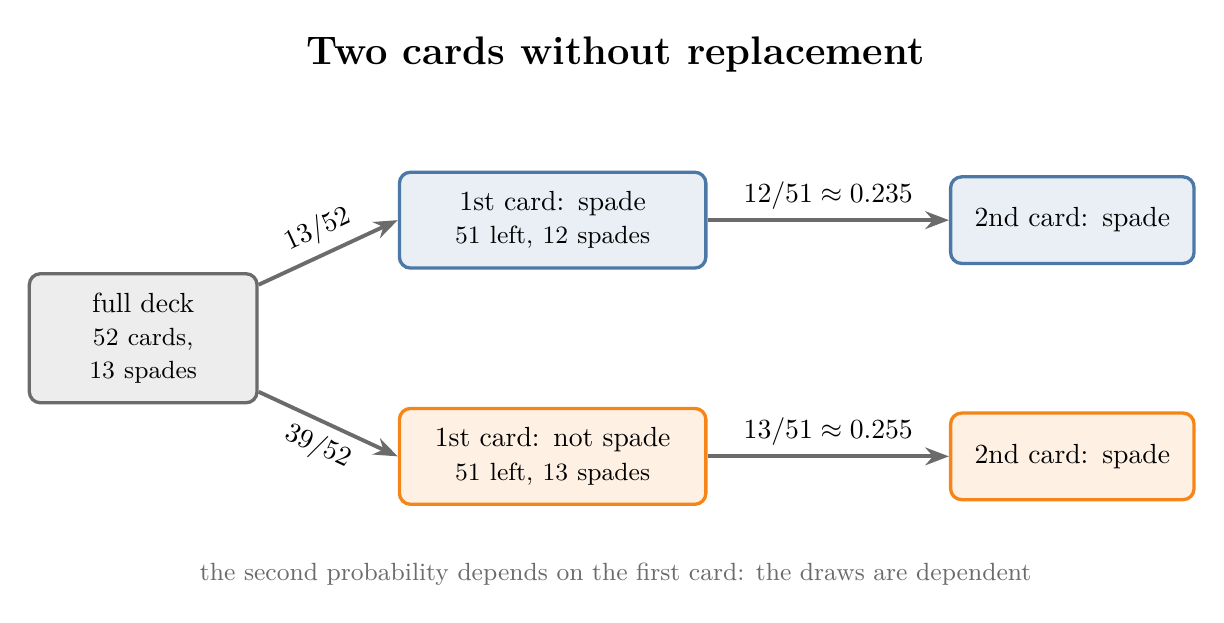
\begin{tikzpicture}[x=1cm, y=1cm]
  \node[title] at (6,3.6) {Two cards without replacement};
  \node[box=cgrey, text width=2.4cm] (deck) at (0,0) {full deck\\ \small 52 cards, 13 spades};
  \node[box=cblue, text width=3.4cm] (s1) at (5.2,1.5) {1st card: spade\\ \small 51 left, 12 spades};
  \node[box=corange, text width=3.4cm] (n1) at (5.2,-1.5) {1st card: not spade\\ \small 51 left, 13 spades};
  \node[box=cblue, text width=2.6cm] (s2) at (11.8,1.5) {2nd card: spade};
  \node[box=corange, text width=2.6cm] (n2) at (11.8,-1.5) {2nd card: spade};
  \draw[arrow] (deck) -- node[above, sloped] {$13/52$} (s1.west);
  \draw[arrow] (deck) -- node[below, sloped] {$39/52$} (n1.west);
  \draw[arrow] (s1) -- node[above] {$12/51 \approx 0.235$} (s2);
  \draw[arrow] (n1) -- node[above] {$13/51 \approx 0.255$} (n2);
  \node[note] at (6,-3.0) {the second probability depends on the first card: the draws are dependent};
\end{tikzpicture}
\end{document}
